\section{Evaluation}

\subsection{Comparison with linear Kalman Filter}
We train two sets of \gls{gp}s on the trajectories from both the heuristic and semantic trackers, one for each topic.
First, we split the ground truth trajectories into two sets for training and testing.
Then we match both sets of trajectories with ground truth, as described in \S\ref{sec:tracker-eval}. 
For both trajectories that matched to the same ground truth, the training data are from the bounding boxes on the frames appear in both trajectories.
Therefore, two sets of \gls{gp}s have the same amount of training data. 
The \gls{gp}s are trained incrementally, with a randomly sampled trajectory at a time.
This simulates the process of our tracker setting.
Apart from \gls{gp}s trained on different datasets, we also compare with the Klaman filter with a linear dynamic model.
A Kalman filter is built with the ground truth as measurement. 
It is the best that a linear Kalman filter can achieve since the measurement given is the perfect ground truth.
\ref{fig:gp-iou} shows change of the mean \gls{iou} with the trajectory count.
The \gls{gp}s start with one training trajectories, where they make a poor prediction on the testing data.
However, with a few more trajectories, the \gls{gp}s have much better performance.
The dash and solid lines are \gls{gp}s from the heuristic and semantic trackers, separately. 
The \gls{gp}s trained on the trajectories of the semantic tracker generally have better prediction over the ones from the heuristic tracker.
By comparing with the linear Kalman filter, the \gls{gp}s significantly perform better.
The \gls{gp}s, for topic 0 have the most significant gap with the baseline Kalman filter. 
From \ref{fig:entry-exit-full-0}, the vehicles from topic 0 moving with a increasing size and experience the nonlinearity the most; \gls{gp} captures such non-linear change.
\begin{figure}
\centering
    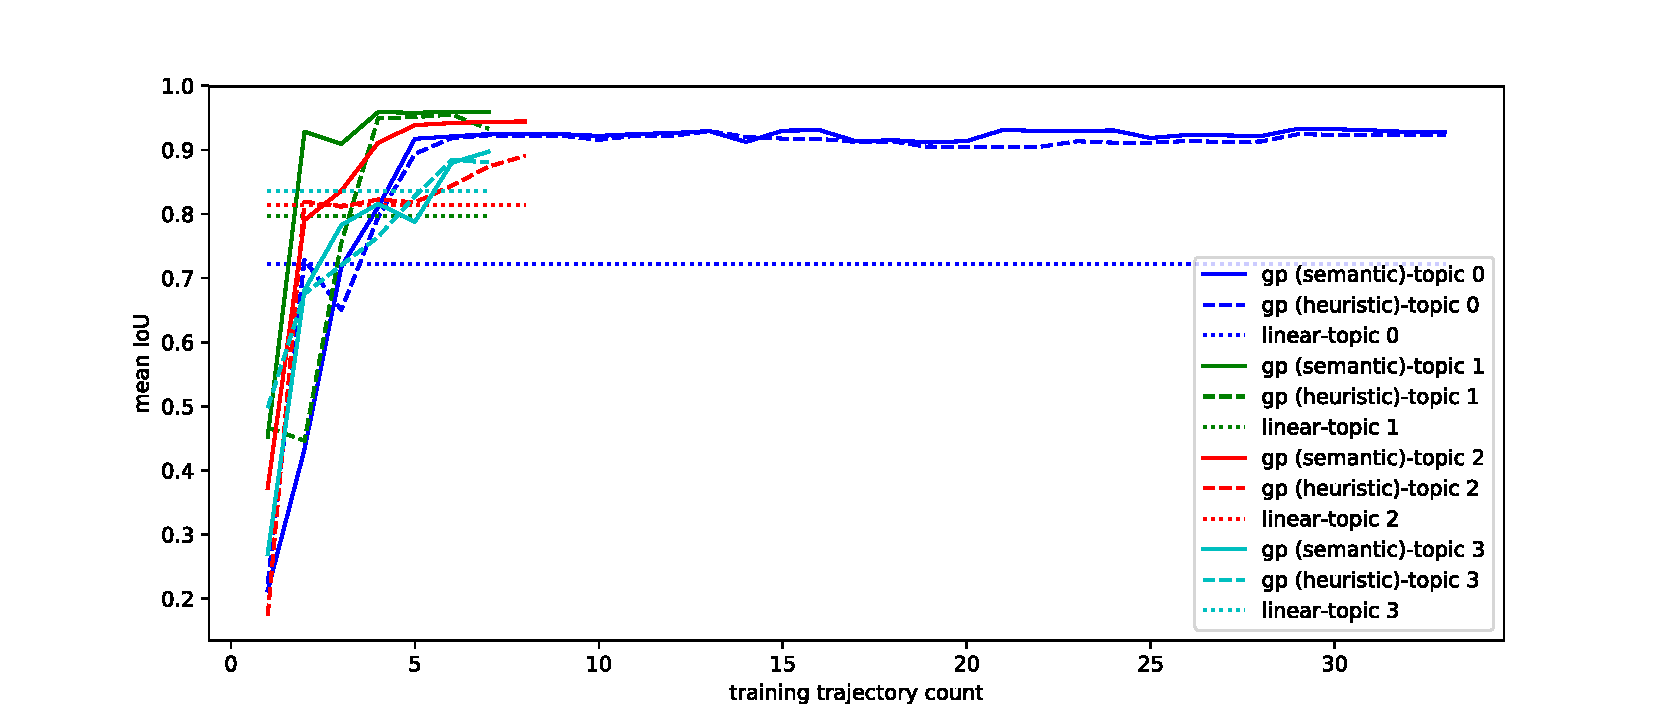
\includegraphics[width=\linewidth]{./img/gp/gp-iou.pdf}
    \caption{The mean IoU of \gls{gp}s trained on the trajectories from the heuristic and semantic tracker, and the linear Kalman filter. Each topic has two \gls{gp}s and a linear Kalman filter.}
    \label{fig:gp-iou}
\end{figure}

\subsection{Case study}
\ref{fig:kf-gp-1}, \ref{fig:kf-gp-2}, \ref{fig:kf-gp-3} shows the comparison of the Kalman filter with linear and non-linear model, which we call KF (left) and GP-UKF (right). Under projection, vehicles moving towards the right of the frame has an increasing rate of size and velocity. 
In \ref{fig:kf-gp-1}, tracking just started. GP-UKF tracker does not have any training data, which works similarly with the KF tracker. 
In \ref{fig:kf-gp-2}, GP-UKF has accumulated 1-2 trajectories, showing a slightly better coverage of the actual vehicle. 
Finally, when GP-UKF has 5-8 trajectories as the training data, GP-UFK adapts to the scale and velocity significantly better than linear KF tracker in \ref{fig:kf-gp-3}.

\begin{figure}[!ht]
\centering
    \begin{subfigure}{0.43\linewidth}
        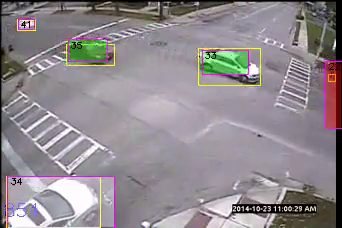
\includegraphics[width=\linewidth]{./img/gp/193402-kf-1.png}
        \subcaption{Kalman filter with Linear model.}
        \label{subfig:kf-1}
    \end{subfigure}
    \begin{subfigure}{0.43\linewidth}
        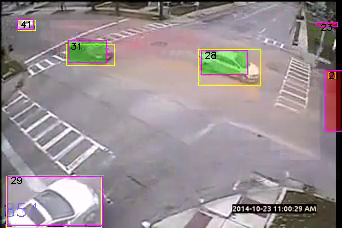
\includegraphics[width=\linewidth]{./img/gp/193402-gp-1.png}
        \subcaption{Kalman filter with non-linear model.}
        \label{subfig:gp-1}
    \end{subfigure}%
    \caption{Tracking screenshots at frame 854, no trajectory for Gaussian Process.}
    \label{fig:kf-gp-1}
\end{figure}

\begin{figure}
\centering
    \begin{subfigure}{0.43\linewidth}
        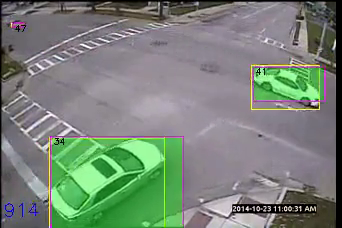
\includegraphics[width=\linewidth]{./img/gp/193402-kf-2.png}
        \subcaption{Kalman filter with linear model.}
        \label{subfig:kf-2}
    \end{subfigure}
    \begin{subfigure}{0.43\linewidth}
        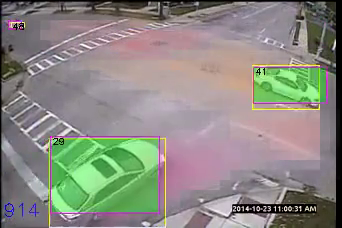
\includegraphics[width=\linewidth]{./img/gp/193402-gp-2.png}
        \subcaption{Kalman filter with non-linear model.}
        \label{subfig:gp-2}
    \end{subfigure}%
    \caption{Tracking screenshots at frame 914, 1-2 trajectories for Gaussian Process.}
    \label{fig:kf-gp-2}
\end{figure}

\begin{figure}
\centering
    \begin{subfigure}{0.43\linewidth}
        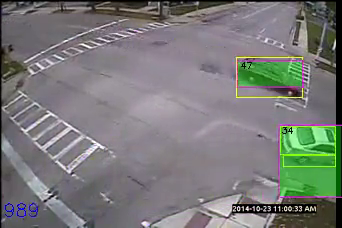
\includegraphics[width=\linewidth]{./img/gp/193402-kf-3.png}
        \subcaption{Kalman filter with linear model.}
        \label{subfig:kf-3}
    \end{subfigure}
    \begin{subfigure}{0.43\linewidth}
        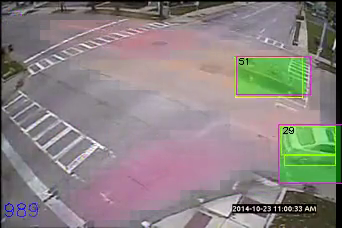
\includegraphics[width=\linewidth]{./img/gp/193402-gp-3.png}
        \subcaption{Kalman filter with non-linear model.}
        \label{subfig:gp-3}
    \end{subfigure}%
    \caption{Tracking screenshots at frame 989, 5-8 trajectories for Gaussian Process.}
    \label{fig:kf-gp-3}
\end{figure}